% Data Model
\begin{figure}[htb]
    \centering
    %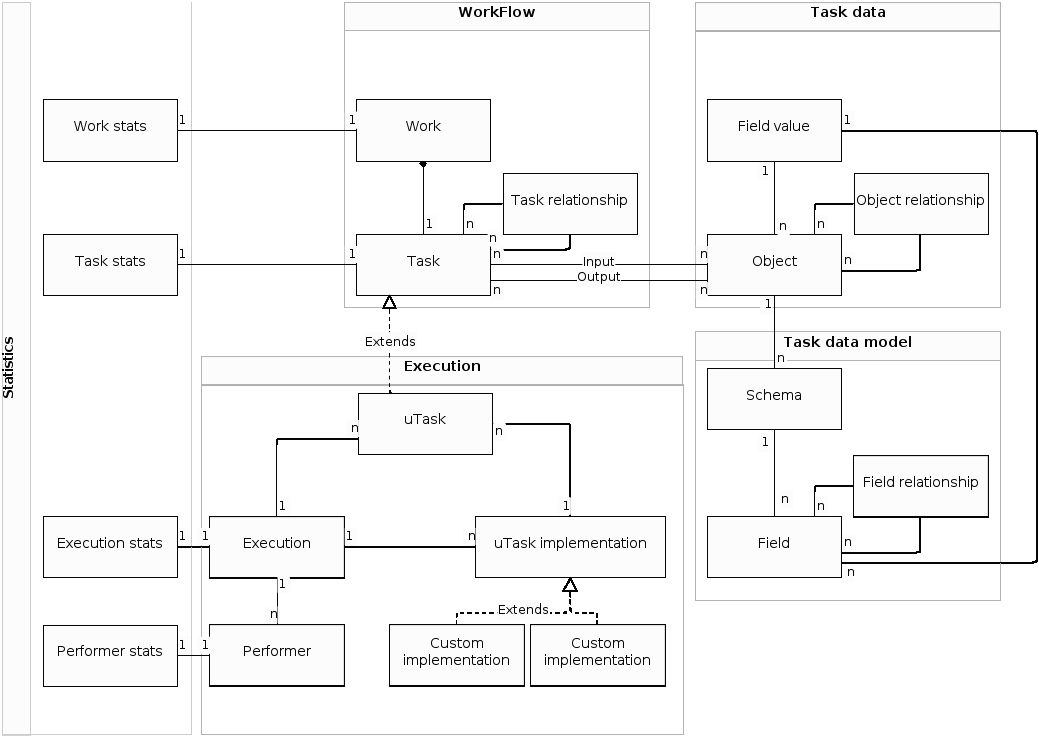
\includegraphics[width=\textwidth]{DataModel.png}
    \hspace{-7em}
    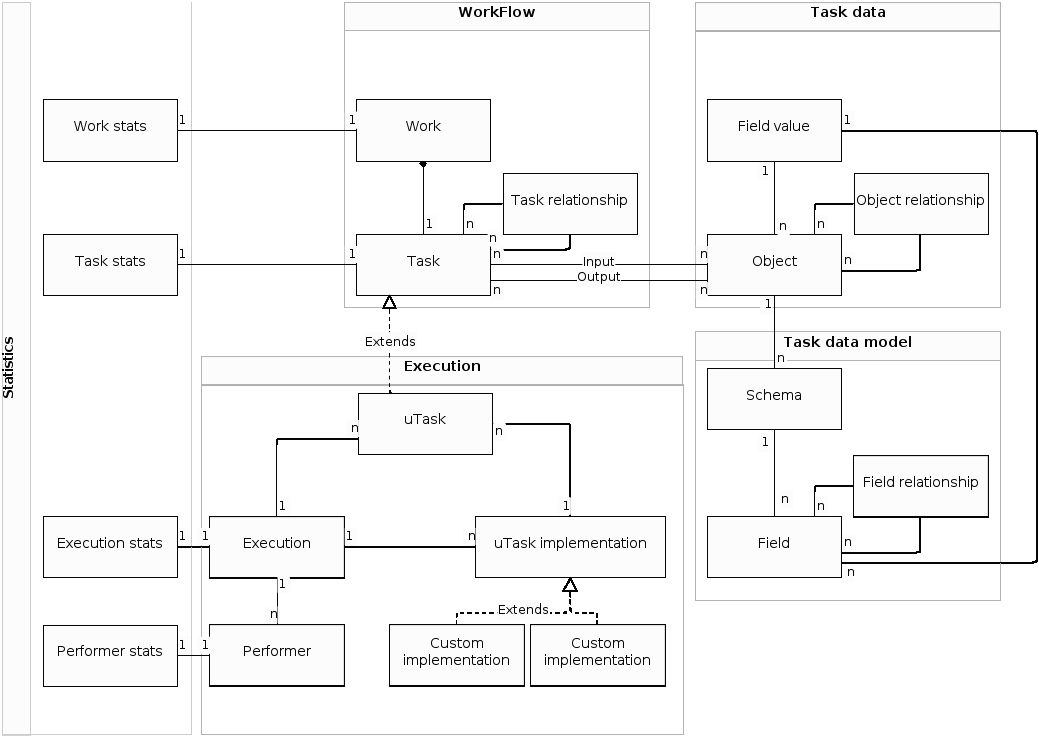
\includegraphics[width=1.3\columnwidth]{DataModel.png}
    \caption{Data Model.}
    \label{fig:data-model}
\end{figure}
In this section, we define the \emph{Data model} of the System. All the components
used in the \emph{Architectural model} leverage on the flexibility of this model.
The data model is composed of 5 parts that together give the conceptual view
of a human computation and automatic computation platform.

\begin{description}
	\item[The WorkFlow] contains the
\end{description}

% task con custom proiperties in modo da configurare i runtime